\subsection{User Interface}%
\label{sec:ui-implementation}
%
The UI implementation consists of various \textbf{XML files complemented with java code}. Consequently, one can consider the UI features and present images related to those rather than simply overload the document with XML code. Firstly, as one enters the app, an initial screen is presented (figure \ref{fig:app-overview} - \textbf{1}), in this screen the app checks for if the phone supports the Bluetooth services necessary to run the application and requests user permission to enable Bluetooth (figure \ref{fig:app-overview} - \textbf{2}). The second and main screen of the app is composed of a navigation drawer (figure \ref{fig:app-overview} - \textbf{4}) and a screen with two buttons for initiating the video stream (figure \ref{fig:app-overview} - \textbf{3}). The navigation drawer is the place where the user can perform all the communication-related actions like enabling Wifi or setting up a Wi-fi or Bluetooth connection. The aforesaid main screen also as has a status indicator. As one enters the rover control screen (figure \ref{fig:app-overview} - \textbf{11}) the orientation is automatically changed to the one (preemptively defined) that allows the correct initial position for the car control. In this screen, one can see the RVVS' live transmission and the speed and wheel tilt percentages sent to the same module. The video allows the fullscreen display (figure \ref{fig:app-overview} - \textbf{9,10,12}), still showing the latter percentages as a periodic pop-up (figure \ref{fig:app-overview} - \textbf{9}). Note that one tried to achieve a balance between app functionality while also creating a user-friendly environment.
%
\begin{figure}[!ht]
\centering
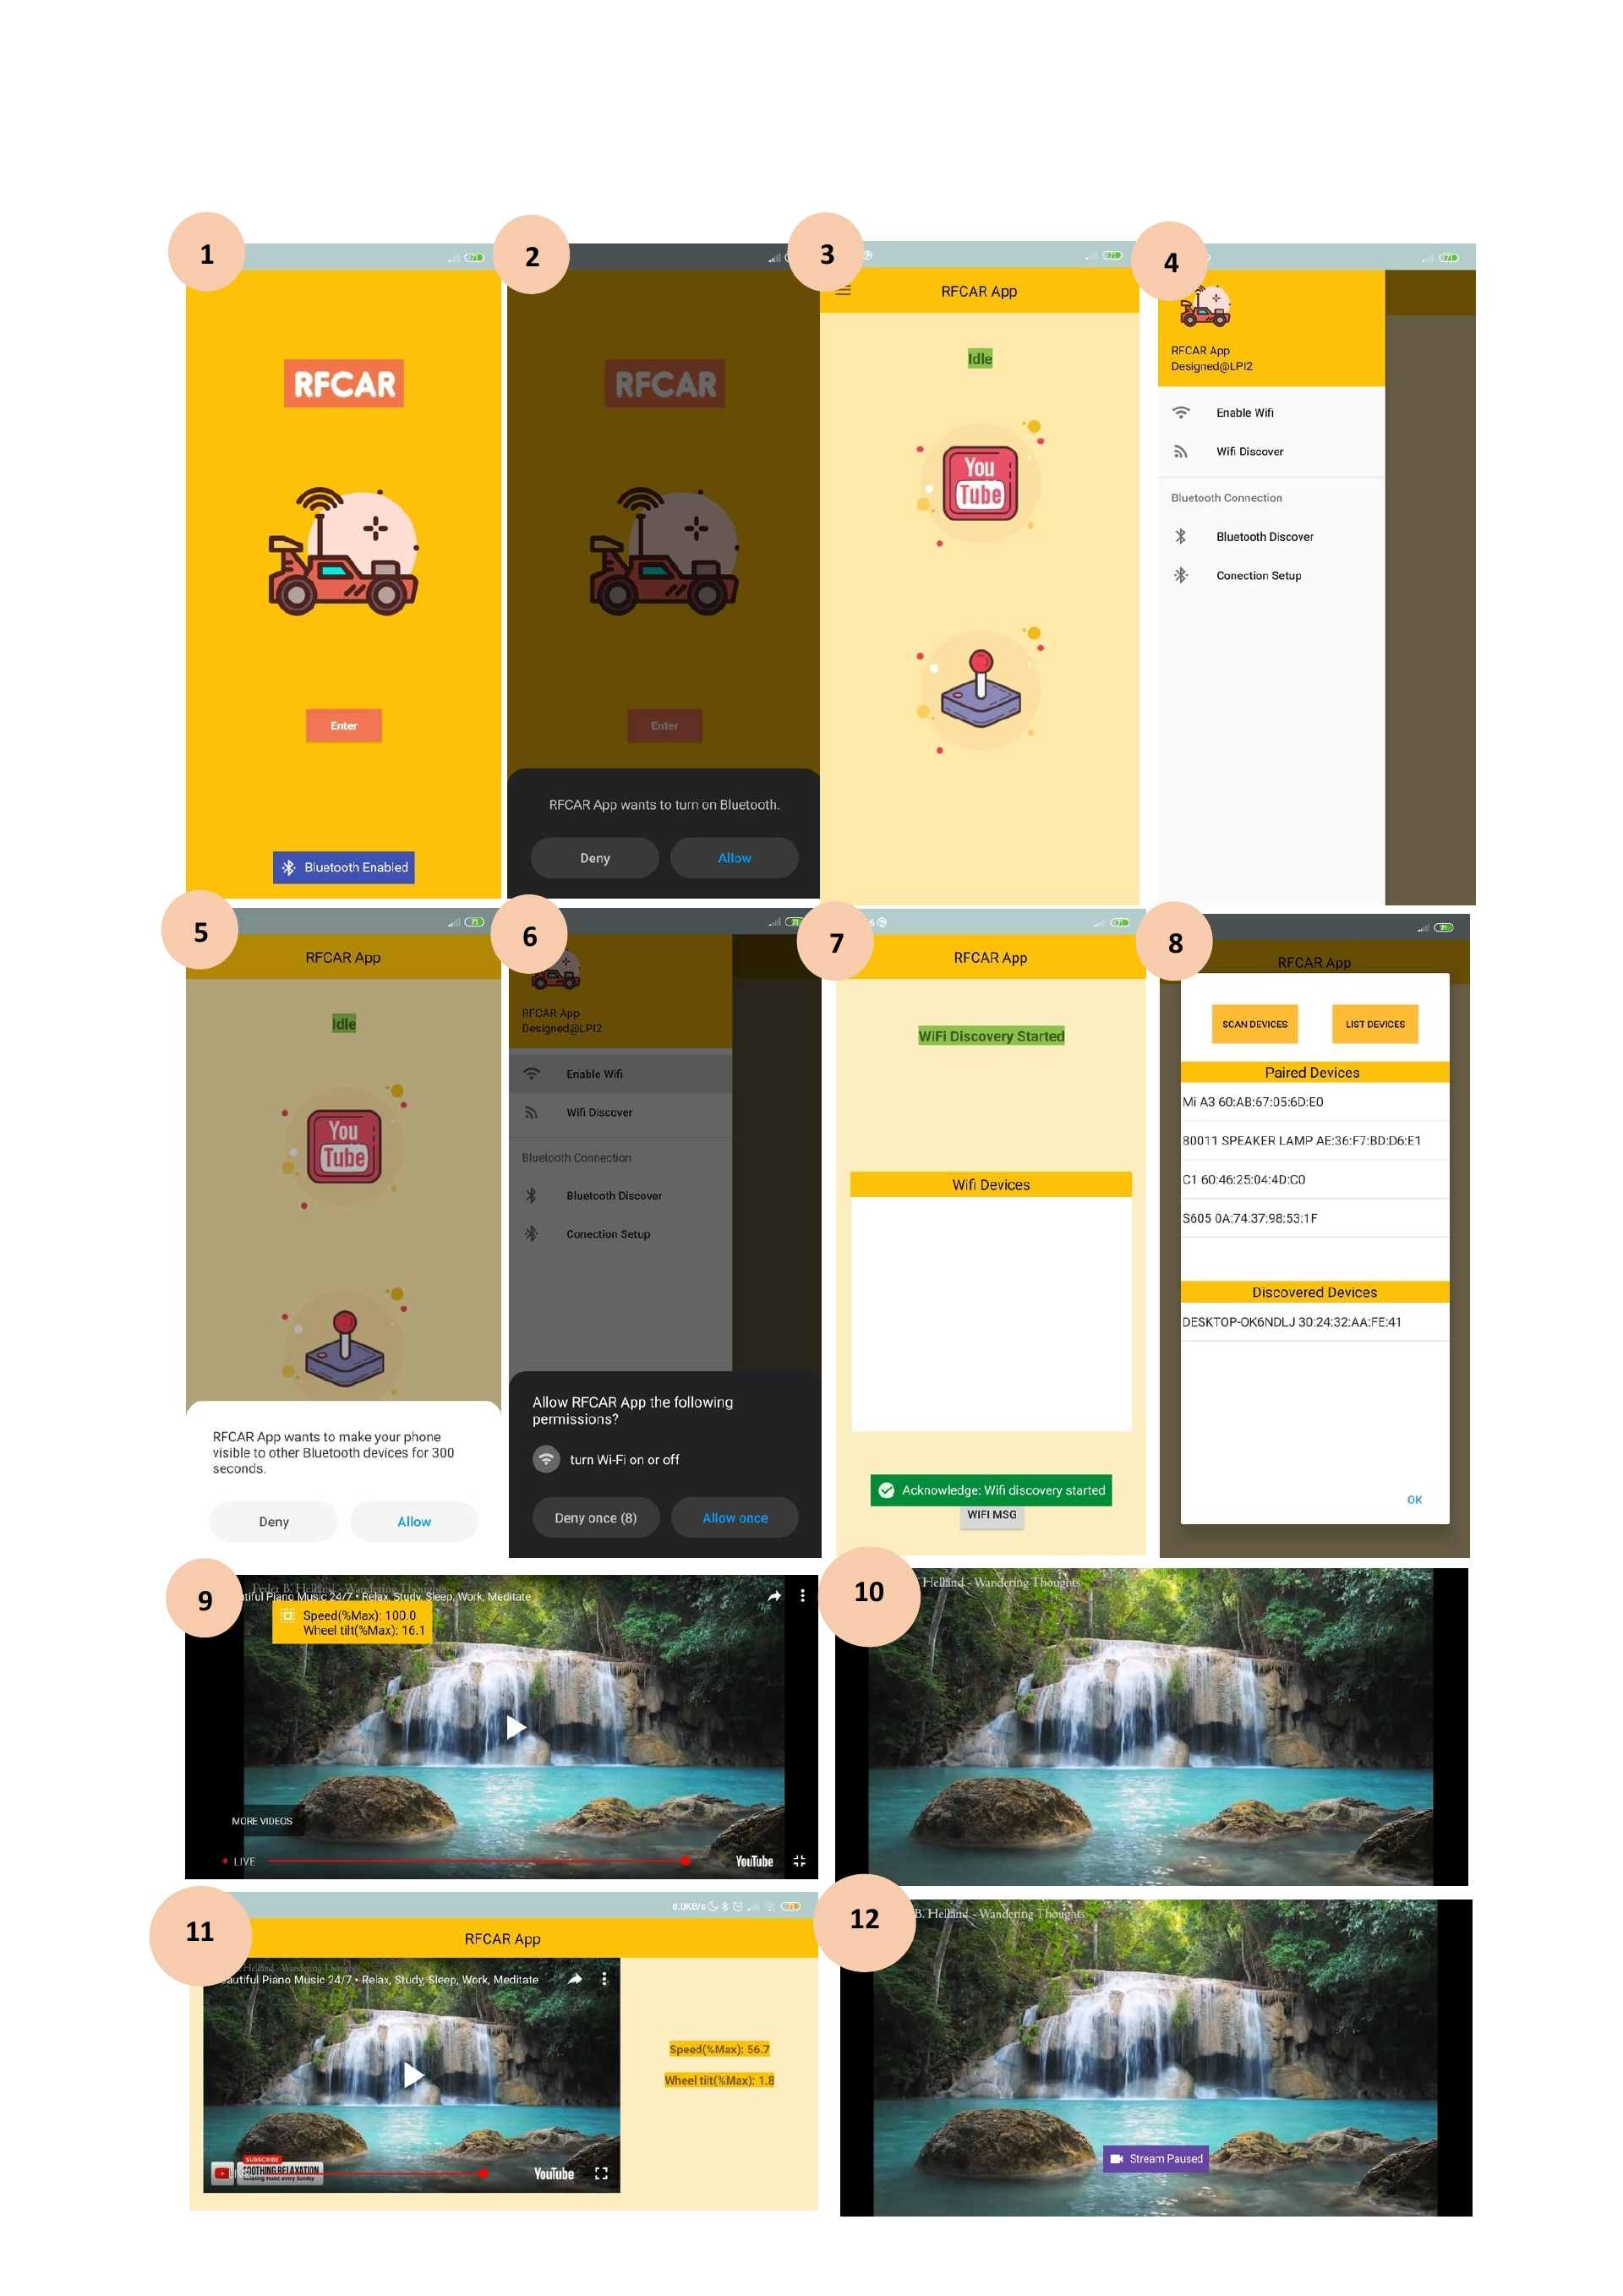
\includegraphics[width=0.85\textwidth]{img/general-app-overview.jpg}
\caption{\label{fig:app-overview}General App Overview}
\end{figure}
%